\documentclass[times, 12pt, utf8]{article}
\RequirePackage[utf8]{inputenc}
\RequirePackage[croatian]{babel}

\usepackage{hyperref, url}
\usepackage{enumitem}
\usepackage{titlesec}
\usepackage{graphics}
\usepackage{graphicx}
\usepackage{xcolor}

% Image location
\graphicspath{ {../misc/} }

%xcolor configuration
\definecolor{darkBlue}{HTML}{171f68}

%hyperref configuration
\hypersetup{
    colorlinks=true,
    linkcolor=black,
    filecolor=magenta,      
    urlcolor=darkBlue
}

% titlesec configuration
\titleformat{\section}{
	\normalfont\Large\bfseries
}{\thesection}{1em}{}

\titleformat{\subsection}{
	\normalfont\large\bfseries\raggedright
}{}{0em}{\underline}[]

\begin{document}

\begin{titlepage}
    \clearpage
    \thispagestyle{empty}
    \pagenumbering{gobble}

    \title{
    {\large Projekt iz programske potpore} \\
    { \textbf{Bioinformatika - Poravnavnaje i mapiranje sekvenci genoma} }

    \vbox{}
    \vspace{0.5cm}

    \footnotesize{
        \begin{itemize}[leftmargin=3.5cm]
            \setlength{\itemindent}{0.8cm}

            Voditelji: 
                \item[-] Prof. dr. sc. Mile Šikić
                \item[-] Mag. ing. Rober Vaser
        \end{itemize}
        
        }
        
        \date{}
        }

    \clearpage
\end{titlepage}

\maketitle

\newpage
\clearpage
\pagenumbering{gobble}

\tableofcontents

\newpage
\clearpage
\pagenumbering{arabic}

\section{Uvod}
    U sklopu predmeta 'Projekt iz programske potpore' na Sveučilištu u Zagrebu,
    Fakultet elektrotehnike i računarstva, studenti u međusobnoj suradnji 
    pod nadzorom profesora i asistenata rješavaju praktične probleme
    s ciljem upoznavanja alata i tehnika korištenih u struci. Grupa 
    okupljena pod vodstvom prof. dr. sc. Mile Šikića bavi se 
    poravnavanjem i mapiranja genoma koristeći moderni C++,
    sustav za upravljene izvornim kodom (eng. version control) git,
    automatizirani sustav izgradnje (eng. build system) CMake,
    sustav kontinuirane integracije TravisCI.
    Po završetku projekta, studenti bi trebali stječi vještine 
    korištenja spomenutih tehnologija te ujedno biti u stanju 
    implementirati osnovne algoritme iz područja bioinformatike.

\section{Rad na projektu}

    Prije početka rada na projektu, studenti su dužni proći 
    navedene lekcije ako nisu upoznati sa zadanim tehnologijama: 
    \\ \indent 
        \href
            {http://www.cplusplus.com/doc/tutorial/}
            {C++}
        , \href
            {http://rogerdudler.github.io/git-guide/}
            {GitHub}
        , \href 
            {https://cmake.org/cmake-tutorial/}
            {CMake}
        , \href
            {https://github.com/google/googletest/blob/master/googletest/docs/primer.md}
            {GoogleTest}
        , \href
            {https://docs.travis-ci.com/user/getting-started/}
            {TravisCI} \\ \\
    Također, poželjno je pridržavati se 
    \href {https://google.github.io/styleguide/cppguide.html}{Googleovih smjernica}
        za pisanje i oblikovanje C++ koda.
        Po početku rada studenti su podjelljeni u timove: blue, orange, pink i brown.
        \footnote{\href {https://en.wikipedia.org/wiki/Reservoir_Dogs}{White?}}
        Svaki tim ima svoju git granu i dozvoljeno je kreiranje novih s imanovanjem 
        formata: \colorbox{gray!30}{'white\_feature\_one'}.

    \subsubsection{Cilj}
        Studenti će implementirati biblioteku koja podržava nekoliko algoritama
        za mapiranje velikog broja relativno malih podnizova znakova na veliki 
        niz znakova koji predstavlja referentni genom. Cilj je povezati
        implementirane biblioteke u jedan program, obično nazvan eng. mapper, 
        s ciljem poravnanja skeniranih sekvenci.

        \begin{figure}[h]
            \centering
            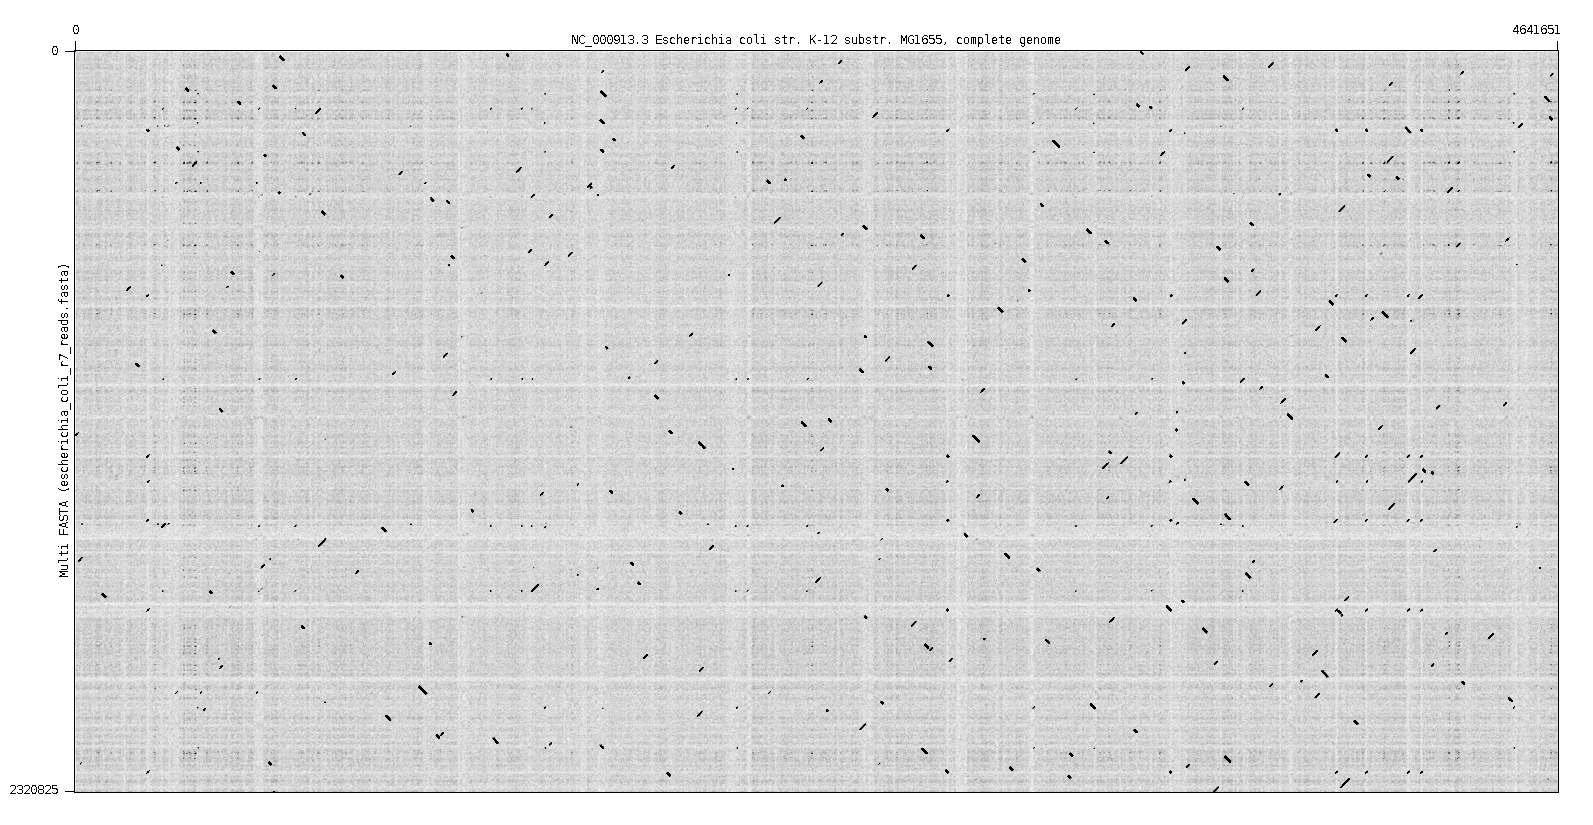
\includegraphics[width=\textwidth]{sample_mappings.png}
            \caption{Vizualni prikaz}
        \end{figure}

    \subsection{Zadaci}
        \subsubsection{Alati, okruženje, učitavanje podataka}
            Svaki tim dužan je držati README.md svoje grane usklađenim 
            s README.md glavne (eng. master) grane. Kao uvod u projekt,
            svaki tim treba postaviti strukturu projekta i inicijalizirati
            CMake postavke za izgradnju glavnog programa s imenom formata 
            \colorbox{gray!30}{$<$ime tima$>$\_mapper} (npr. \colorbox{gray!30}{white\_mapper})
            Program preko naredbene konzole mora prihvatiti dva argumenta:
            put do skeniranih sekvenci i put do referendnog genoma.



        \subsubsection{Poravnanaje sekvenci}
        \subsubsection{DNA Minimizeri}
        \subsubsection{Mapiranje sekvenci}

\subsection{Rezultati}

\section{Literatura}

        \begin{itemize}
            \item[--] \href
                {https://www.fer.unizg.hr/_download/repository/bioinformatika_skripta_v1.2.pdf}
                {FER - Bioinformatika}
        \end{itemize}

\end{document}